\section{Resultados}
\label{sec:resultados}

\subsection{Qué se midió}

23 grupos, 65\,185 decisiones, 3\,564 celdas. El detalle por modelo y dataset:

\begin{table}[t]
\centering
\caption{Los 23 grupos medidos: cada fila cruza un modelo con un dataset, con su cardinalidad $n$, el número
de ítems y la accuracy observada. La última columna confirma \texttt{output\_tokens} $= 0$ en todos los
casos, es decir, ninguno genera texto.}
\label{tab:grupos}
{\footnotesize
\setlength{\tabcolsep}{3pt}
\resizebox{\columnwidth}{!}{%
\begin{tabular}{p{0.36\columnwidth}p{0.30\columnwidth}lll l}
\toprule
modelo & dataset & $n$ & ítems & accuracy & tokens \\
\midrule
\texttt{Qwen/\allowbreak Qwen3.5-0.8B-Base} & \texttt{banking77} & 77 & 3\,076 & 0.0156 & 0 \\
\texttt{Qwen/\allowbreak Qwen3.5-0.8B-Base} & \texttt{clinc150} & 151 & 3\,100 & 0.0387 & 0 \\
\texttt{Qwen/\allowbreak Qwen3.5-0.8B-Base} & \texttt{sst5} & 5 & 1\,101 & 0.2116 & 0 \\
\texttt{Qwen/\allowbreak Qwen3.5-0.8B-Base} & \texttt{typed-\allowbreak decisions} & 2, 4, 5 & 2\,000 & 0.4860 & 0 \\
\texttt{Qwen/\allowbreak Qwen3.5-0.8B-Base} & \texttt{wanli} & 3 & 5\,000 & 0.3598 & 0 \\
\texttt{convaiinnovations/\allowbreak laya} & \texttt{banking77} & 77 & 3\,076 & 0.3765 & 0 \\
\texttt{convaiinnovations/\allowbreak laya} & \texttt{sst5} & 5 & 1\,101 & 0.3451 & 0 \\
\texttt{convaiinnovations/\allowbreak laya} & \texttt{typed-\allowbreak decisions} & 2, 4, 5 & 2\,000 & 0.3595 & 0 \\
\texttt{convaiinnovations/\allowbreak laya} & \texttt{wanli} & 3 & 5\,000 & 0.6178 & 0 \\
\texttt{convaiinnovations/\allowbreak laya/\allowbreak multilingual} & \texttt{banking77} & 77 & 3\,076 & 0.3560 & 0 \\
\texttt{convaiinnovations/\allowbreak laya/\allowbreak multilingual} & \texttt{clinc150} & 151 & 3\,100 & 0.6274 & 0 \\
\texttt{convaiinnovations/\allowbreak laya/\allowbreak multilingual} & \texttt{sst5} & 5 & 1\,101 & 0.2489 & 0 \\
\texttt{convaiinnovations/\allowbreak laya/\allowbreak multilingual} & \texttt{typed-\allowbreak decisions} & 2, 4, 5 & 2\,000 & 0.3515 & 0 \\
\texttt{convaiinnovations/\allowbreak laya/\allowbreak multilingual} & \texttt{wanli} & 3 & 5\,000 & 0.5750 & 0 \\
\texttt{convaiinnovations/\allowbreak laya/\allowbreak typed-decisions} & \texttt{banking77} & 77 & 3\,076 & 0.3781 & 0 \\
\texttt{convaiinnovations/\allowbreak laya/\allowbreak typed-decisions} & \texttt{clinc150} & 151 & 3\,100 & 0.4732 & 0 \\
\texttt{convaiinnovations/\allowbreak laya/\allowbreak typed-decisions} & \texttt{sst5} & 5 & 1\,101 & 0.4505 & 0 \\
\texttt{convaiinnovations/\allowbreak laya/\allowbreak typed-decisions} & \texttt{typed-\allowbreak decisions} & 2, 4, 5 & 2\,000 & 0.7685 & 0 \\
\texttt{convaiinnovations/\allowbreak laya/\allowbreak typed-decisions} & \texttt{wanli} & 3 & 5\,000 & 0.6190 & 0 \\
\texttt{jaredpalmer/\allowbreak kev-0.8b} & \texttt{banking77} & 77 & 3\,076 & 0.8134 & 0 \\
\texttt{jaredpalmer/\allowbreak kev-0.8b} & \texttt{sst5} & 5 & 1\,101 & 0.4995 & 0 \\
\texttt{jaredpalmer/\allowbreak kev-0.8b} & \texttt{typed-\allowbreak decisions} & 2, 4, 5 & 2\,000 & 0.4595 & 0 \\
\texttt{jaredpalmer/\allowbreak kev-0.8b} & \texttt{wanli} & 3 & 5\,000 & 0.5954 & 0 \\
\bottomrule
\end{tabular}}}
\end{table}

Un dato aparte que el ecosistema no reporta: en cardinalidad alta, \textbf{Kev-0.8B saca 0.813 de accuracy
en \texttt{banking77} ($n = 77$) frente a 0.377 del checkpoint base de Laya}. El ecosistema sí entrena para
muchas opciones; no todos los modelos por igual.

\begin{figure}[t]
\centering
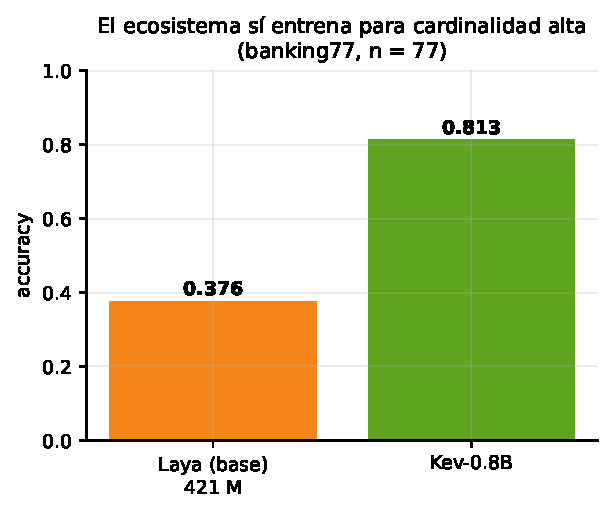
\includegraphics[width=\columnwidth]{fig7-accuracy-banking77}
\caption{Accuracy en \texttt{banking77} ($n = 77$) por configuración: Kev-0.8B (0.813) duplica al mejor
checkpoint de Laya (0.378) y triplica al checkpoint base (0.377). El ecosistema sí entrena para
cardinalidad alta, pero no todos los modelos por igual.}
\label{fig:accuracy-banking77}
\end{figure}

\subsection{El objeto de la tesis, en una cifra}

Sobre las \textbf{65\,185} distribuciones medidas (una fila por decisión), la diferencia entre la definición
de \texttt{confidence} más alta y la más baja de la \textbf{misma} distribución tiene:

\begin{table}[t]
\centering
\caption{Brecha interna de \texttt{confidence} sobre las 65\,185 distribuciones medidas: diferencia entre la
definición más alta y la más baja de una \emph{misma} distribución.}
\label{tab:brecha}
{\small
\setlength{\tabcolsep}{4pt}
\begin{tabular}{lr}
\toprule
estadístico & valor \\
\midrule
mediana & \textbf{0.288} \\
percentil 90 & \textbf{0.434} \\
máximo & \textbf{0.848} \\
\bottomrule
\end{tabular}}
\end{table}

Es decir: en el caso típico, dos implementaciones del mismo campo discrepan en casi tres décimas sobre el
mismo dato, y el peor caso llega a 0.85. Cualquier umbral fijado sobre una de las dos no significa lo mismo
sobre la otra.

\begin{figure}[t]
\centering
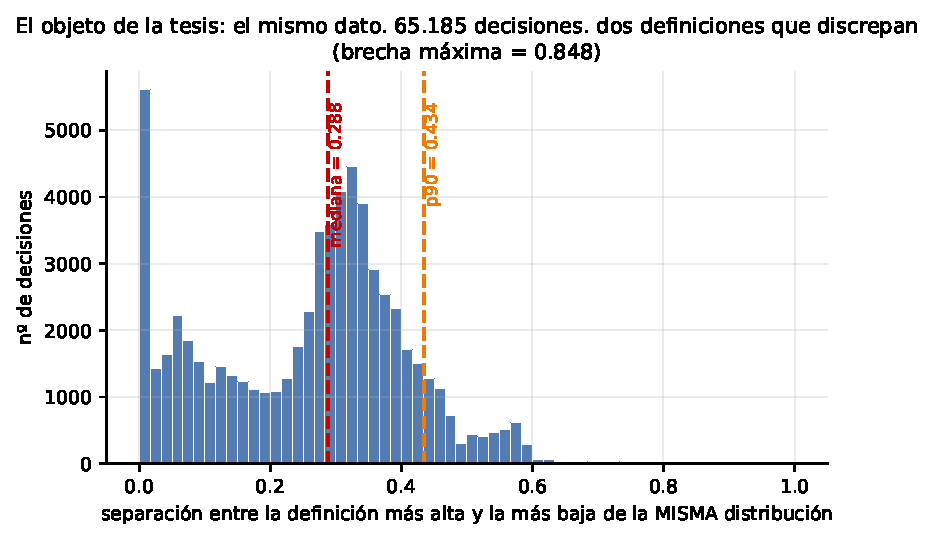
\includegraphics[width=\columnwidth]{fig1-brecha}
\caption{La cifra central: sobre las 65\,185 decisiones medidas, la definición más alta y la más baja de
\texttt{confidence} difieren con mediana 0.288 y alcance máximo 0.848. Un umbral fijado con una definición
no significa lo mismo con la otra.}
\label{fig:brecha}
\end{figure}

\subsection{El número no viaja; el mapa sí}

El titular es sobre el \textbf{nivel principal \texttt{raw}}, que es el que congela el pre-registro. En él,
de las 3\,564 celdas, \textbf{348 tienen mapa cerrado} entre definiciones (misma clase de equivalencia y
misma cardinalidad; 1\,044 si se cuentan los tres niveles), que son las únicas donde tiene sentido comparar
el porte directo contra el porte con mapa. El error absoluto medio:

\begin{table}[t]
\centering
\caption{Error absoluto medio del porte directo frente al porte con mapa, por subconjunto de celdas (nivel
\texttt{raw}). El porte directo se equivoca hasta dos órdenes de magnitud más que el porte con mapa.}
\label{tab:error-transferencia}
{\footnotesize
\setlength{\tabcolsep}{3pt}
\begin{tabular}{p{0.34\columnwidth}rlll}
\toprule
subconjunto & celdas & $\lvert\Delta\rvert$ directo & $\lvert\Delta\rvert$ con mapa & factor \\
\midrule
todas las celdas con mapa & 348 & 0.2528 & 0.0123 & 20.5$\times$ \\
\textbf{sin empates dominantes en el umbral} & \textbf{312} & \textbf{0.2337} & \textbf{0.0021} & \textbf{109.2$\times$} \\
solo modelos entrenados (sin control crudo) & 276 & 0.2289 & 0.0020 & 112.8$\times$ \\
solo $n = 2$ (Proposición 3) & 180 & 0.3006 & 0.0218 & 13.8$\times$ \\
solo $n \ge 3$ (Proposición 1) & 168 & 0.2015 & 0.0021 & 95.8$\times$ \\
nivel \texttt{L0} (debiasing sin etiquetas) & 324 & 0.2190 & 0.0059 & 37.1$\times$ \\
nivel \texttt{L1} (temperatura con etiquetas) & 312 & 0.3022 & 0.0024 & 126.0$\times$ \\
\bottomrule
\end{tabular}}
\end{table}

El porte directo se equivoca \textbf{del orden de cien veces más} que el porte con mapa. El matiz de la
tercera columna lo explica §5.4.

\begin{figure}[t]
\centering
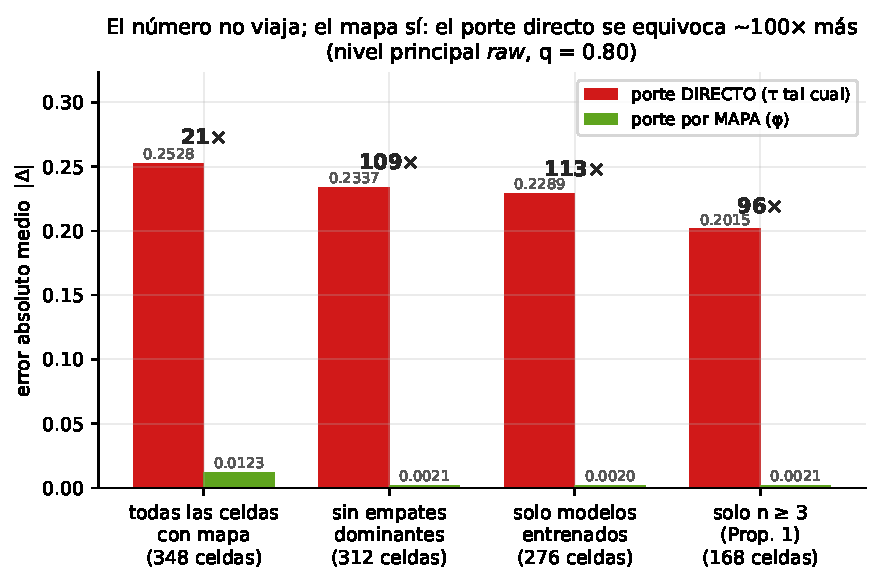
\includegraphics[width=\columnwidth]{fig2-directo-vs-mapa}
\caption{El titular: el porte directo del umbral (sin transformar) se equivoca del orden de cien veces más
que el porte con el mapa cerrado cuando este existe (0.2337 frente a 0.0021 sin empates dominantes).}
\label{fig:directo-vs-mapa}
\end{figure}

\textbf{Cómo leer la tabla.} El porte con mapa tiene un suelo que no es culpa del mapa: si el umbral cae
sobre un valor \textbf{empatado} en muchas salidas (modelos saturados), la cobertura salta y ni el mapa
puede dar $q$ exacto. Por eso la comparación limpia es la del subconjunto sin empates dominantes (masa por
debajo del 5\,\%), y por eso \texttt{delta\_mapa} debe leerse contra \texttt{delta} de la \textbf{misma}
celda, nunca como un cero absoluto. La columna \texttt{n\_empates\_tau} de la matriz declara, en cada celda,
cuántos ítems comparten el umbral.

\begin{figure}[t]
\centering
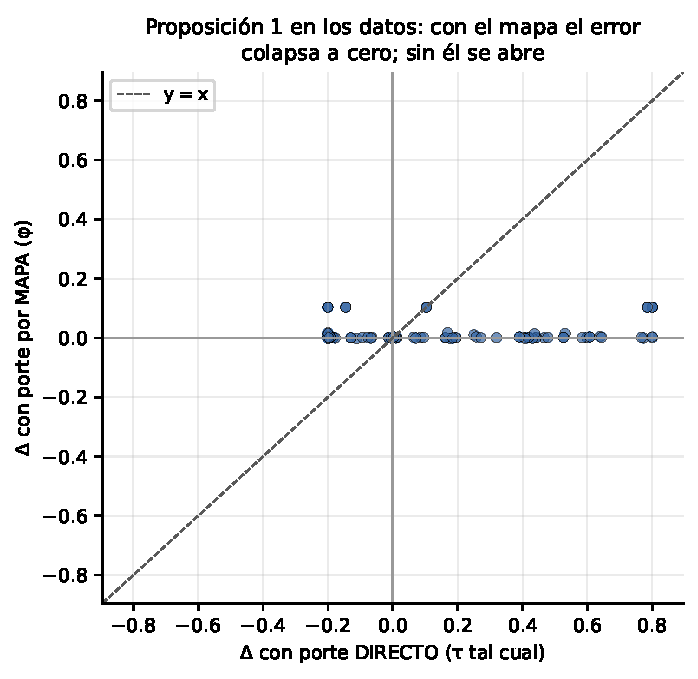
\includegraphics[width=\columnwidth]{fig3-delta-vs-mapa}
\caption{La Proposición 1 sobre los datos: celda a celda, la caída de cobertura del porte directo ($\lvert\Delta\rvert$ directo) contra la del porte con mapa. Con el mapa el error colapsa al suelo que imponen
los empates del umbral, no el mapa.}
\label{fig:delta-vs-mapa}
\end{figure}

\subsection{El promedio no es el resumen: la estructura está en el par}

La distribución de $\Delta$ es \textbf{bimodal}: hay pares de definiciones que coinciden y pares que fallan
en grande. El titular es el par, no la media global.

\begin{table}[t]
\centering
\caption{Caída de cobertura por par de definiciones (origen $A$ $\to$ destino $B$), ordenada por la mediana.
La mediana del par manda sobre la media global: el promedio engaña.}
\label{tab:par}
{\footnotesize
\setlength{\tabcolsep}{3pt}
\begin{tabular}{lrrrl}
\toprule
$A \to B$ & celdas & $\lvert\Delta\rvert$ mediana & $\lvert\Delta\rvert$ media & ¿mapa? \\
\midrule
\texttt{margin} $\to$ \texttt{jev} & 15 & \textbf{0.0023} & 0.0250 & sí \\
\texttt{jev} $\to$ \texttt{margin} & 15 & \textbf{0.0023} & 0.0293 & sí \\
\texttt{jev} $\to$ \texttt{pmax} & 99 & \textbf{0.0759} & 0.1568 & sí \\
\texttt{ent} $\to$ \texttt{jev} & 15 & \textbf{0.1837} & 0.1898 & sí \\
\texttt{ent} $\to$ \texttt{margin} & 15 & \textbf{0.1837} & 0.1898 & sí \\
\texttt{margin} $\to$ \texttt{pmax} & 15 & \textbf{0.2000} & 0.2253 & sí \\
\texttt{ent} $\to$ \texttt{pmax} & 15 & \textbf{0.2000} & 0.2421 & sí \\
\texttt{pmax} $\to$ \texttt{jev} & 99 & \textbf{0.2574} & 0.2973 & sí \\
\texttt{margin} $\to$ \texttt{ent} & 15 & \textbf{0.3474} & 0.3855 & sí \\
\texttt{jev} $\to$ \texttt{ent} & 15 & \textbf{0.3474} & 0.3857 & sí \\
\texttt{pmax} $\to$ \texttt{margin} & 15 & \textbf{0.5262} & 0.5154 & sí \\
\texttt{pmax} $\to$ \texttt{ent} & 15 & \textbf{0.7667} & 0.6787 & sí \\
\bottomrule
\end{tabular}}
\end{table}

Dos de las coincidencias son \textbf{identidades matemáticas}, no azar: (i) a $n = 2$, $C_{\text{Jev}}$ y
$C_{\text{mar}}$ son la \textbf{misma} función ($2\cdot p_{\max} - 1$), así que su porte directo ya da casi
cero; (ii) a cardinalidad alta, $C_{\text{Jev}} = (n\cdot p - 1)/(n - 1) \to p$, así que \texttt{jev} y
\texttt{pmax} convergen y sus umbrales casi coinciden. En el extremo opuesto,
$\text{pmax} \to \text{ent}$ es el peor par: no cambia la escala, cambia la \textbf{forma} de la función.

\begin{figure}[t]
\centering
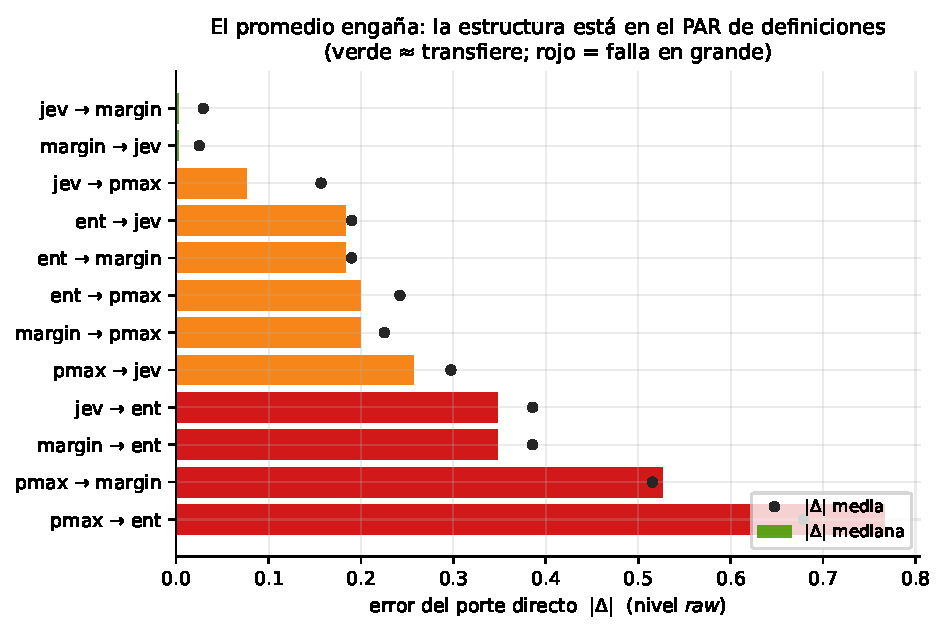
\includegraphics[width=\columnwidth]{fig4-por-par}
\caption{El promedio engaña: la estructura está en el par. Hay pares de definiciones que coinciden por
identidad matemática (medianas de 0.0023) y pares que fallan en grande (hasta 0.7667), y la media global
borra esa bimodalidad.}
\label{fig:por-par}
\end{figure}

Fracción de celdas que transfieren bien ($\lvert\Delta\rvert < 0.01$), por cardinalidad (nivel \texttt{raw}):

\begin{table}[t]
\centering
\caption{Fracción de celdas que transfieren bien ($\lvert\Delta\rvert < 0.01$) según la cardinalidad $n$. El
umbral solo viaja a cardinalidad alta.}
\label{tab:cardinalidad}
{\footnotesize
\setlength{\tabcolsep}{3pt}
\begin{tabular}{lrrl}
\toprule
$n$ & celdas con mapa & $\lvert\Delta\rvert$ mediana & \% con $\lvert\Delta\rvert < 0.01$ \\
\midrule
2 & 180 & 0.2141 & 14\,\% \\
3 & 30 & 0.1775 & 0\,\% \\
4 & 30 & 0.4085 & 0\,\% \\
5 & 60 & 0.2000 & 0\,\% \\
77 & 30 & 0.0058 & 63\,\% \\
151 & 18 & 0.0127 & 44\,\% \\
\bottomrule
\end{tabular}}
\end{table}

\begin{figure}[t]
\centering
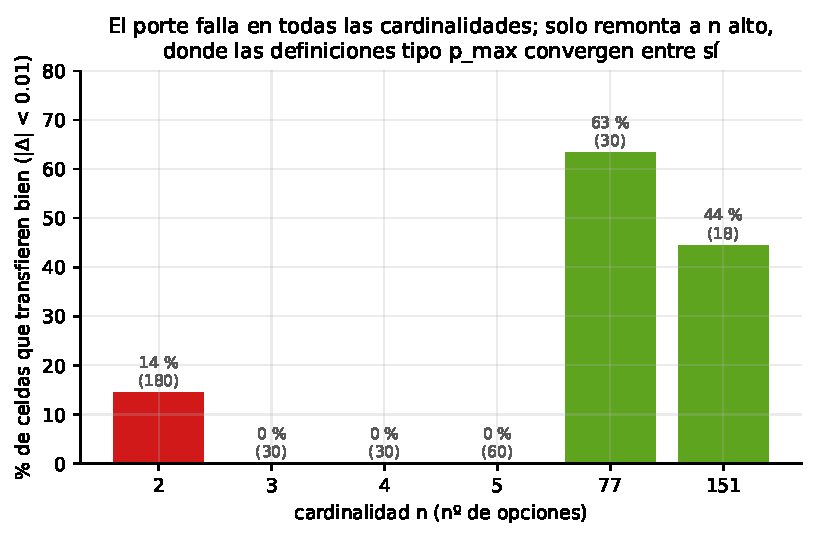
\includegraphics[width=\columnwidth]{fig5-por-cardinalidad}
\caption{Transferencia por cardinalidad $n$ (nivel \texttt{raw}): con $n \le 5$ casi ninguna celda
transfiere bien ($\lvert\Delta\rvert < 0.01$ en el 14\,\% de los casos y menos), mientras que a $n \ge 77$ la
mitad o más lo logra.}
\label{fig:por-cardinalidad}
\end{figure}

\subsection{Efecto de la cardinalidad}

\begin{table}[t]
\centering
\caption{Caída de cobertura y celdas significativas tras FDR, por cardinalidad $n$, con el dataset de
ejemplo. El porte falla en todas las cardinalidades.}
\label{tab:cardinalidad-fdr}
{\footnotesize
\setlength{\tabcolsep}{3pt}
\begin{tabular}{lrrrl}
\toprule
$n$ & celdas & $\lvert\Delta\rvert$ medio & celdas con FDR & dataset de ejemplo \\
\midrule
2 & 60 & 0.3042 & 52 & \texttt{typed-\allowbreak decisions} \\
3 & 60 & 0.2011 & 60 & \texttt{wanli} \\
4 & 60 & 0.3240 & 60 & \texttt{typed-\allowbreak decisions} \\
5 & 120 & 0.2664 & 119 & \texttt{sst5} \\
77 & 60 & 0.1638 & 52 & \texttt{banking77} \\
151 & 36 & 0.2140 & 32 & \texttt{clinc150} \\
\bottomrule
\end{tabular}}
\end{table}

El porte falla en todas las cardinalidades, pero con dos matices ya visibles en §5.4: a $n$ bajo el daño es
grande y sistemático, mientras que a cardinalidad alta ($n \ge 77$) las definiciones tipo $p_{\max}$
convergen entre sí y una parte de las celdas transfiere bien. La Proposición 3 predice que con $n = 2$ todas
las definiciones deberían ser equivalentes en orden; en los datos eso se cumple \textbf{dentro del par
$\text{jev} \leftrightarrow \text{margin}$} (misma función) y no en el resto, porque el porte directo cruza
escalas distintas aunque el orden sea el mismo. Es la distinción entre el número y el mapa.

\subsection{Dónde el umbral no viaja (nivel \texttt{raw}, $q = 0.80$, tras FDR)}

\begin{table}[t]
\centering
\caption{Celdas donde el umbral no viaja: nivel \texttt{raw}, $q = 0.80$, tras FDR. Portar el umbral pierde
toda la cobertura ($\Delta = 0.80$, cobertura B $= 0$) o casi toda.}
\label{tab:no-viaja}
{\footnotesize
\setlength{\tabcolsep}{3pt}
\resizebox{\columnwidth}{!}{%
\begin{tabular}{p{0.38\columnwidth}p{0.30\columnwidth}llrll}
\toprule
modelo & dataset & $n$ & $A \to B$ & $\Delta$ & IC95\,\% & cobertura B \\
\midrule
\texttt{Qwen/\allowbreak Qwen3.5-0.8B-Base} & \texttt{banking77} & 77 & \texttt{ent} $\to$ \texttt{margin} & 0.8000 & [0.800, 0.800] & 0.000 \\
\texttt{Qwen/\allowbreak Qwen3.5-0.8B-Base} & \texttt{sst5} & 5 & \texttt{pmax} $\to$ \texttt{ent} & 0.8000 & [0.800, 0.800] & 0.000 \\
\texttt{Qwen/\allowbreak Qwen3.5-0.8B-Base} & \texttt{typed-\allowbreak decisions} & 2 & \texttt{pmax} $\to$ \texttt{jev} & 0.8000 & [0.800, 0.800] & 0.000 \\
\texttt{Qwen/\allowbreak Qwen3.5-0.8B-Base} & \texttt{typed-\allowbreak decisions} & 2 & \texttt{pmax} $\to$ \texttt{ent} & 0.8000 & [0.800, 0.800] & 0.000 \\
\texttt{Qwen/\allowbreak Qwen3.5-0.8B-Base} & \texttt{typed-\allowbreak decisions} & 2 & \texttt{pmax} $\to$ \texttt{margin} & 0.8000 & [0.800, 0.800] & 0.000 \\
\texttt{convaiinnovations/\allowbreak laya/\allowbreak typed-decisions} & \texttt{typed-\allowbreak decisions} & 2 & \texttt{pmax} $\to$ \texttt{ent} & 0.8000 & [0.800, 0.800] & 0.000 \\
\texttt{jaredpalmer/\allowbreak kev-0.8b} & \texttt{typed-\allowbreak decisions} & 2 & \texttt{pmax} $\to$ \texttt{ent} & 0.8000 & [0.800, 0.800] & 0.000 \\
\texttt{Qwen/\allowbreak Qwen3.5-0.8B-Base} & \texttt{banking77} & 77 & \texttt{pmax} $\to$ \texttt{margin} & 0.7997 & [0.799, 0.800] & 0.000 \\
\texttt{Qwen/\allowbreak Qwen3.5-0.8B-Base} & \texttt{banking77} & 77 & \texttt{ent} $\to$ \texttt{jev} & 0.7997 & [0.799, 0.800] & 0.000 \\
\texttt{Qwen/\allowbreak Qwen3.5-0.8B-Base} & \texttt{banking77} & 77 & \texttt{jev} $\to$ \texttt{margin} & 0.7993 & [0.798, 0.800] & 0.001 \\
\texttt{Qwen/\allowbreak Qwen3.5-0.8B-Base} & \texttt{banking77} & 77 & \texttt{ent} $\to$ \texttt{pmax} & 0.7990 & [0.798, 0.800] & 0.001 \\
\texttt{Qwen/\allowbreak Qwen3.5-0.8B-Base} & \texttt{sst5} & 5 & \texttt{pmax} $\to$ \texttt{margin} & 0.7974 & [0.794, 0.800] & 0.003 \\
\bottomrule
\end{tabular}}}
\end{table}

La lectura es directa: hay celdas en las que portar el umbral \textbf{pierde toda la cobertura}. Quien
calibra al 80\,\% con una definición y despliega con otra puede terminar actuando en el 0\,\% de los casos
(o en todos), sin ningún aviso del modelo.

\begin{figure}[t]
\centering
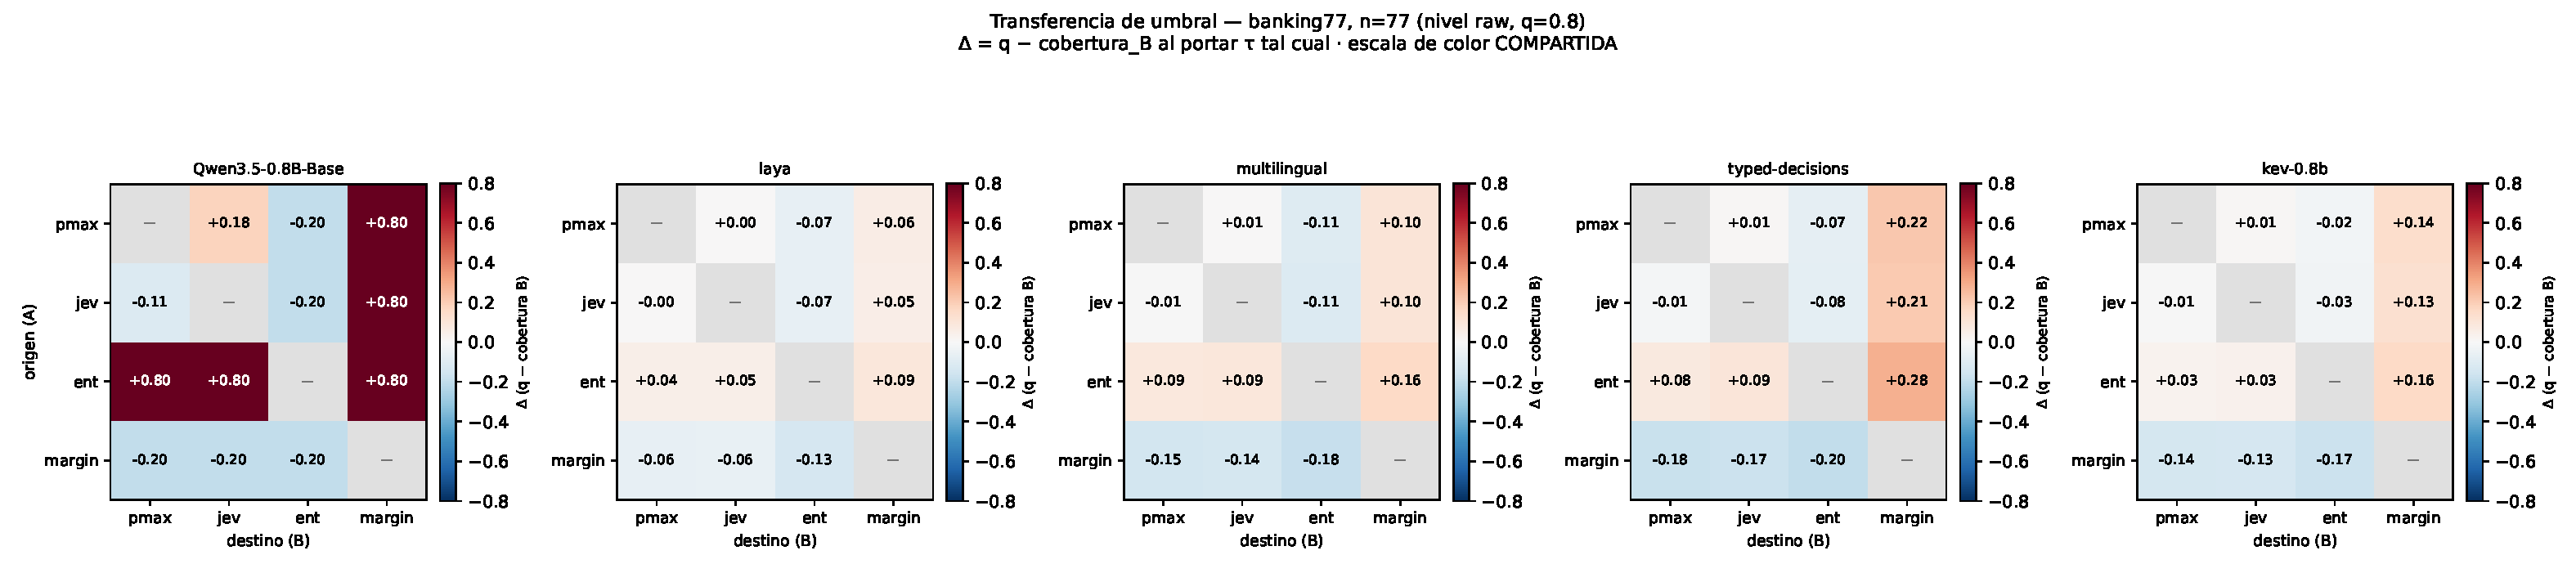
\includegraphics[width=\columnwidth]{fig8-heatmap-banking77}
\caption{Dónde el umbral no viaja: mapa de calor de la caída de cobertura en \texttt{banking77} ($n = 77$,
nivel \texttt{raw}), con filas de definición origen y columnas de definición destino. Cuando el modelo está
saturado, celdas enteras pierden toda la cobertura al cambiar de definición.}
\label{fig:heatmap-banking77}
\end{figure}

\subsection{Hallazgos de metrología del paso 0 (contexto)}

La corrida de verificación sobre \texttt{typed-decisions} dejó, además, dos resultados que no estaban en la
literatura del ecosistema y que son parte del instrumento:

\begin{enumerate}
\item \textbf{La \texttt{choice\_confidence} de Kev es la fórmula de Jev.}
   $(p_{\max} - 1/K)/(1 - 1/K) \equiv (K\cdot p_{\max} - 1)/(K - 1)$, verificado numéricamente para
   $K \in \{2,3,4,7,12\}$. Estaban registradas como definiciones distintas; por la Proposición 1, ese par
   transfiere el umbral de forma exacta.
\item \textbf{El campo \texttt{output\_tokens} tiene tres significados.} Jev y Laya lo reportan como 0 (no
   hay generación); Kev lo usa como recuento de tokens de la respuesta serializada (869\,310 en las mismas
   2\,000 decisiones). Es metrología del propio campo, no un fallo de Kev.
\end{enumerate}

Y sobre la misma corrida, el ECE cambia por completo según la definición: en \texttt{laya-typed-decisions}
va de \textbf{0.216} con $p_{\max}$ a \textbf{0.577} con la entropía normalizada, un factor
\textbf{2.7$\times$} sobre el mismo dato.

\begin{figure}[t]
\centering
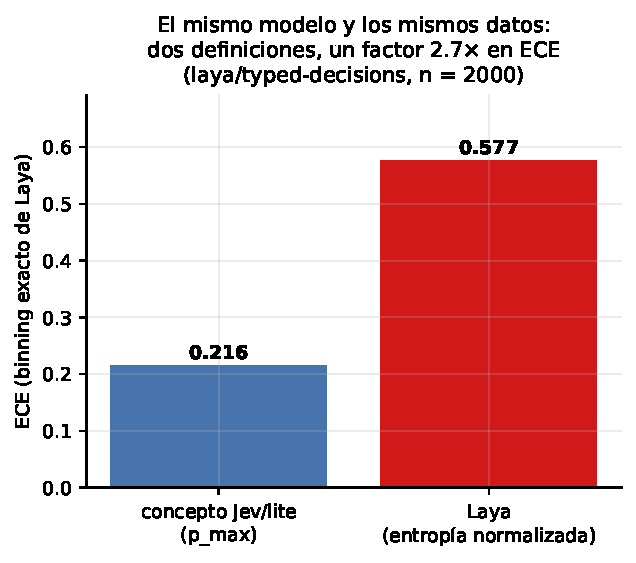
\includegraphics[width=\columnwidth]{fig6-ece-por-definicion}
\caption[El mismo ECE cambia con la definición de \texttt{confidence}]{El mismo dato, dos ECE: en
\texttt{laya-typed-decisions} el ECE va de 0.216 con $p_{\max}$ a 0.577
con la entropía normalizada, un factor 2.7$\times$. El ECE auto-reportado no es una propiedad del modelo
sino de la definición elegida.}
\label{fig:ece}
\end{figure}

\subsection{Extensiones declaradas (posteriores al pre-registro)}

Las cifras de las subsecciones anteriores están selladas por el pre-registro
\texttt{10.5281/zenodo.23266795}: \textbf{23 grupos, 65\,185 decisiones, 3\,564 celdas}. Las dos mediciones de
esta subsección son \textbf{posteriores} a ese pre-registro y se declaran aparte para no moverlas: no recalculan
la matriz sellada ni las filas crudas, se calculan como post-proceso sobre datos ya medidos o sobre un brazo
nuevo, y llevan su fecha.

\subsubsection{Quinta definición del campo: \texttt{conf\_score} (distancia al nivel modal)}

La documentación de TypeSafe define para la primitiva \texttt{score} una \texttt{confidence} que no estaba entre
las cuatro definiciones selladas:
\begin{equation}
\begin{aligned}
C_{\text{score}} &= \max\Bigl(0,\; 1 - \tfrac{1}{M}\,{\textstyle\sum_i}\, p_i\,\lvert i-m\rvert\Bigr),\\
M &= \tfrac{1}{n}\,{\textstyle\sum_i}\, \bigl\lvert i-\tfrac{n-1}{2}\bigr\rvert ,
\end{aligned}
\end{equation}
donde $M$ es la desviación absoluta media de la rejilla uniforme (\emph{MAD} uniforme) y $m$ el nivel modal.
No es una variante de $C_{\text{jev}}$: $C_{\text{jev}}$ mide \textbf{concentración en el máximo};
$C_{\text{score}}$ mide \textbf{dispersión alrededor del nivel modal}. Dos distribuciones con el mismo $p_{\max}$
dan valores distintos. Y es \textbf{ordinal}: exige que los niveles tengan orden y distancia, así que solo se
mide donde el orden existe.

\begin{table}[t]
\centering
\caption{La quinta definición sobre \texttt{sst5} (5 niveles ordinales, 5 configuraciones, 5\,505 decisiones).
La brecha es la diferencia entre la definición más alta y la más baja de la \emph{misma} distribución; el ECE se
calcula sobre la misma corrida y la misma etiqueta de corrección que las otras cuatro.}
\label{tab:extension-score}
{\footnotesize
\begin{tabular}{@{}lr@{}}
\toprule
Brecha, mediana con 4 definiciones & 0.272 \\
Brecha, mediana con 5 definiciones & \textbf{0.290} (p90 0.411, máx 0.581) \\
\midrule
ECE global, $C_{\text{pmax}}$ & 0.204 \\
ECE global, $C_{\text{jev}}$ & 0.184 \\
ECE global, $C_{\text{ent}}$ & 0.199 \\
ECE global, $C_{\text{mar}}$ & 0.237 \\
ECE global, $C_{\text{score}}$ & \textbf{0.241} \\
\midrule
Verificación contra el servicio real & $\lvert\Delta\rvert \le 0.0050$ en 800 filas \\
\bottomrule
\end{tabular}}
\end{table}

\textbf{Por qué solo \texttt{sst5}.} En \texttt{banking77} (77), \texttt{clinc150} (151) y
\texttt{typed-decisions} (2, 4, 5) las etiquetas son nominales: el índice $i$ no significa nada y usarlo sería
añadir un supuesto, no medir. En \texttt{wanli} (3) el orden es discutible. Se declara el límite en lugar de
inventar la escala.

\textbf{El hallazgo que añade.} La quinta definición \textbf{no tiene un sesgo estable}: es la más baja de las
cinco en el \textbf{70.3\,\%} de las filas del control crudo Qwen y la más alta en el \textbf{92.6\,\%} de las de
Laya-multilingual. El signo de la discrepancia depende del modelo, no de la definición --- que es exactamente el
objeto de este trabajo, ahora con una definición más en la lista.

\subsubsection{Brazo pagado: el modelo detrás del campo}

Hasta aquí todo se midió sobre pesos abiertos. El servicio real de TypeSafe (\texttt{jev-1.13.0}, una petición
por ítem) se midió sobre los mismos cinco datasets y se publica como brazo aparte: \textbf{14\,277 decisiones},
gasto \textbf{USD 0.79}, con \texttt{probabilities} y \texttt{confidence} redondeadas a \textbf{0.01} por el
servicio.

\begin{table}[t]
\centering
\caption{Brazo pagado: el servicio real sobre los cinco datasets etiquetados. La última columna es el contador
\texttt{output\_tokens} que reporta el servicio; en todos los brazos de pesos abiertos ese mismo contador vale
cero.}
\label{tab:brazo-pagado}
{\footnotesize
\setlength{\tabcolsep}{4pt}
\begin{tabular}{@{}lrrrr@{}}
\toprule
dataset & $n$ & ítems & accuracy & tokens de salida \\
\midrule
\texttt{banking77} & 77 & 3\,076 & 0.796 & 2\,547\,728 \\
\texttt{clinc150} & 151 & 3\,100 & 0.901 & 4\,034\,486 \\
\texttt{sst5} & 5 & 1\,101 & 0.541 & 19\,818 \\
\texttt{typed-decisions} & 2, 4, 5 & 2\,000 & 0.733 & 270\,290 \\
\texttt{wanli} & 3 & 5\,000 & 0.754 & 220\,650 \\
\bottomrule
\end{tabular}}
\end{table}

Dos observaciones de metrología del propio campo. (i) El contador \texttt{output\_tokens} \textbf{no es cero} en
el servicio (7\,092\,972 en total), a diferencia de los brazos de pesos abiertos: el campo \emph{tokens de
salida} no distingue por sí solo un modelo de decisión de uno generativo; esa lectura solo vale donde se controla
la implementación. (ii) La confianza que el servicio \textbf{devuelve} coincide con la definición que la
especificación le asigna a cada primitiva: $C_{\text{score}}$ en las filas \texttt{score} ($\lvert\Delta\rvert
\le 0.0050$ sobre 800 filas) y $C_{\text{jev}}$ en las de \texttt{choice} (600 filas). La especificación describe
el servicio real, no una reconstrucción.

Sumado a los brazos abiertos, el conjunto tiene \textbf{79\,462 decisiones} y una brecha mediana de
\textbf{0.273} (p90 0.435) --- el mismo orden que la cifra sellada de 0.288, ahora con seis modelos.

\textbf{El porte del umbral con la rejilla de 0.01.} Error absoluto medio del porte sobre las celdas con mapa
cerrado (nivel \texttt{raw}, las tres $q$; 420 celdas):

\begin{table}[t]
\centering
\caption{Porte del umbral en el conjunto combinado, por modelo. La última columna es la fracción media de ítems de
prueba que comparten el umbral (empates inducidos por la rejilla de 0.01 del servicio).}
\label{tab:porte-pagado}
{\footnotesize
\setlength{\tabcolsep}{3pt}
\resizebox{\columnwidth}{!}{%
\begin{tabular}{@{}lrrrr@{}}
\toprule
modelo & celdas & $\lvert\Delta\rvert$ directo & $\lvert\Delta\rvert$ con mapa & factor \\
\midrule
\texttt{typesafe-ai/jev} & 72 & 0.1735 & \textbf{0.0130} & 13.4$\times$ \\
\texttt{laya/multilingual} & 72 & \textbf{0.1315} & 0.0018 & 75.1$\times$ \\
\texttt{laya} & 66 & 0.2581 & 0.0028 & 91.7$\times$ \\
\texttt{laya/typed-decisions} & 72 & 0.2515 & 0.0014 & 174.4$\times$ \\
\texttt{kev-0.8b} & 66 & 0.2813 & 0.0022 & 128.5$\times$ \\
\texttt{Qwen3.5-0.8B} (control) & 72 & 0.3441 & 0.0517 & 6.7$\times$ \\
\midrule
global & 420 & 0.2392 & 0.0124 & 19.3$\times$ \\
\bottomrule
\end{tabular}}}
\end{table}

La lectura es en dos partes, y la segunda corrige la intuición. (i) El porte \textbf{directo} de Jev (0.1735) es
de los mejores, pero \textbf{no el mejor}: el checkpoint \texttt{laya/multilingual} transfiere mejor (0.1315) sin
ser el modelo de referencia del campo. Comparar $\lvert\Delta\rvert$ directo entre modelos mezcla dos causas ---la
definición y la calidad del modelo--- y por eso el titular de este trabajo es el par de definiciones, no el
modelo. (ii) El porte \textbf{con mapa} de Jev es \textbf{4.6 a 9.3 veces} el de los checkpoints abiertos (0.0130
frente a 0.0014--0.0028) y su factor directo/mapa es \textbf{13.4$\times$}, un orden de magnitud menor que el de
ellos (75--174$\times$). La causa está medida: la rejilla de 0.01 reasigna masa a valores empatados y
\textbf{2.5\,\%} de los ítems de prueba de Jev comparten el umbral, frente a \textbf{0.1\,\%} en los abiertos
(25$\times$), con 4 de 72 celdas por encima del 5\,\% de empate frente a 0 en las abiertas. El mapa cerrado sigue
siendo válido (Proposición~1); lo que la rejilla degrada es la \textbf{resolución del umbral}, no la equivalencia
entre definiciones.

\emph{Fuentes:} \path{results/matrix/EXTENSION_CONF_SCORE.md} y
\path{results/matrix_pagado/RESUMEN_MATRIZ_PAGADO.md}; se regeneran con
\path{src/matriz/extension_conf_score.py} y \path{src/matriz/correr_matriz_pagado.sh}. Ninguna de estas dos
extensiones modifica el nivel \texttt{raw} sellado, ni las 3\,564 celdas, ni las 65\,185 filas crudas.
